\chapter{Architektury přístupových systémů}
\DIFaddbegin 

\DIFaddend Přístupové systémy jsou elektronické systémy řídící přístup uživatelů do omezených prostor v závislosti na jejich prokázané identitě.

\begin{figure}[!h]
    \centering
    \DIFdelbeginFL %DIFDELCMD < 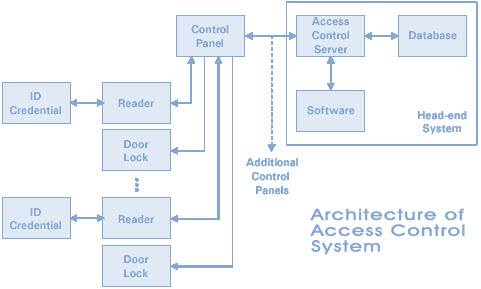
\includegraphics[width=80mm]{Architetcture-of-Access-Control-System}
%DIFDELCMD <     %%%
\DIFdelendFL \DIFaddbeginFL 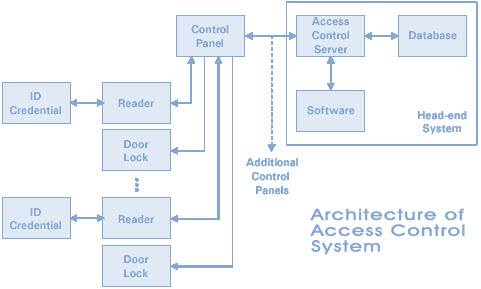
\includegraphics[width=130mm]{Architetcture-of-Access-Control-System}
    \DIFaddendFL \caption{Příklad architektury přístupového systému \cite{accessControlSystem_eiprocus}}
    \label{fig:Access control system architecture}
\end{figure}

Obrázek \ref{fig:Access control system architecture} zobrazuje typickou architekturu přístupového systému, kde ID Credential představuje prvek \DIFdelbegin \DIFdel{ůmožňující }\DIFdelend \DIFaddbegin \DIFadd{umožňující }\DIFaddend identifikovat uživatele, např. RFID tag, otisk prstu nebo QR kód. 
\DIFaddbegin \DIFadd{Zařízení typu }\DIFaddend Reader slouží ke čtení dat z ID Credential a v digitální podobě je \DIFdelbegin \DIFdel{pošle }\DIFdelend \DIFaddbegin \DIFadd{odesílá }\DIFaddend k zařízení typu Control Panel.
Zařízení \DIFaddbegin \DIFadd{typu }\DIFaddend Door Lock řídí fyzický přístup uživatelů do omezených prostor. 
Zařízení typu Control Panel tvoří rozhranní mezi Access Control Server a páry zařízení typů Reader a Door Lock. 
Zařízení typu Control Panel jsou obvykle připojena 
k zařízení typu Access Control Server přes TCP/IP síť \DIFdelbegin \DIFdel{.
A }\DIFdelend \DIFaddbegin \DIFadd{a }\DIFaddend páry zařízení \DIFaddbegin \DIFadd{typů }\DIFaddend Reader a Door Lock jsou obvykle připojeny k zařízení typu Control panel přes RS485 síť\DIFdelbegin \DIFdel{, jehož hlavním účelem je řízení těchto párů}\DIFdelend . Databáze obsahuje \DIFdelbegin \DIFdel{všechny }\DIFdelend \DIFaddbegin \DIFadd{všechna }\DIFaddend uživatelské ID.
Na Access Control Serveru je spuštěn Software (SW) spravující databázi a komunikující se všemi zařízeními typu Contril Panel.
Zařízení typu Reader čte uživatelská ID z předložených ID Credential \DIFdelbegin \DIFdel{uživateli }\DIFdelend a přeposílá je k zařízení typu Control Panel, které je dále přeposílá na Access Control Server. 
Access Control Software vyhledá obdržená uživatelská ID v \DIFdelbegin \DIFdel{databáze }\DIFdelend \DIFaddbegin \DIFadd{databázi }\DIFaddend a pokud je nalezeno, pošle příkaz odpovídajícímu zařízení typu Control Panel k přepnutí odpovídajícímu zařízení typu Door Lock\DIFaddbegin \DIFadd{, čímž je uživateli udělen přístup do omezené oblasti }\DIFaddend \cite{accessControlSystem_eiprocus}.
